\documentclass[hyperref={pdfpagelabels=false}]{beamer}
% beamer already loads hyperref; do NOT load \usepackage{hyperref} again.

\usepackage{ragged2e} % 文字向兩邊對齊
\renewcommand{\raggedright}{\leftskip=0pt \rightskip=0pt plus 0cm}

\usepackage{listings}
\usepackage{lmodern}
\usepackage{fontspec}
\usepackage{xeCJK}
\setCJKmainfont{Noto Sans CJK TC}
%（可選）若你會用到無襯線中文或等寬中文，建議補上：
\setCJKsansfont{Noto Sans CJK TC}
\setCJKmonofont{Noto Sans Mono CJK TC}

\usepackage[english]{babel}
\usepackage{amsmath,amssymb,amsfonts,amsthm}

% hyperref settings (since beamer already loads hyperref)
\hypersetup{
  colorlinks=true,
  urlcolor=blue,
  citecolor=blue,
  pdfborder={0 0 0}
}

\usepackage{accsupp}% http://ctan.org/pkg/accsupp
\newcommand{\emptyaccsupp}[1]{\BeginAccSupp{ActualText={}}#1\EndAccSupp{}}

\usepackage{tikz}
\usetikzlibrary{arrows,decorations.pathmorphing,backgrounds,fit,positioning,shapes.symbols,chains}

\usepackage{booktabs}
\usepackage{threeparttable}
\usepackage{colortbl} 
\usepackage{xcolor}
\usetikzlibrary{tikzmark}

\newcommand{\indep}{\perp\!\!\!\perp}
\newcommand{\nindep}{\not\!\perp\!\!\!\perp}

\beamertemplatefootpagenumber

%-------------------------------------------------------
% Title
%-------------------------------------------------------
\title[Selection Bias \& RCT]{Selection Bias and Randomized Controlled Trial}
\author{Prof. Tzu-Ting Yang \\ 楊子霆}
\institute{Institute of Economics, Academia Sinica \\ 中央研究院經濟研究所}
\date{\today}

% \usetheme{CambridgeUS}
% %\usecolortheme{seahorse}
% \setbeamertemplate{footline}{%
% 	\hfill\usebeamercolor[fg]{page number in head/foot}%
% 	\usebeamerfont{page number in head/foot}%
% 	\insertframenumber\,/\,\inserttotalframenumber\hspace{1em}\vspace{2pt}%
% }

\usetheme{Boadilla}
%\useinnertheme{rectangles}

%\usetheme{CambridgeUS}
\usecolortheme{seahorse}
\setbeamertemplate{footline}{%
	\hfill\usebeamercolor[fg]{page number in head/foot}%
	\usebeamerfont{page number in head/foot}%
	\insertframenumber\,/\,\inserttotalframenumber\hspace{1em}\vspace{2pt}%
}


% \usepackage{beamerthemeshadow}
% %\usecolortheme{seahorse}
% \setbeamertemplate{footline}{%
% 	\hfill\usebeamercolor[fg]{page number in head/foot}%
% 	\usebeamerfont{page number in head/foot}%
% 	\insertframenumber\,/\,\inserttotalframenumber\hspace{1em}\vspace{2pt}%
% }


%\usepackage{beamerthemeshadow}
\beamersetuncovermixins{\opaqueness<1>{25}}{\opaqueness<2->{15}}



\begin{document}
	
	\begin{frame}{}
		\titlepage
	\end{frame}




\begin{frame}{Causal Effect and Counterfactual}
	\begin{itemize}
		
		
		\item In many applications, we might be interested in the ATE or the ATT
				\vspace{0.2cm}
		\item These causal effects are defined by \textbf{comparing potential outcomes}
								\vspace{0.2cm}
		\item But we only know:	
						\vspace{0.2cm}					
				\begin{itemize}
					\item Whether an individual was treated or not
													\vspace{0.2cm}
					\item The \textbf{observed outcome} of the individual
				\end{itemize}
	
		
	\end{itemize}
\end{frame}
    
	
\begin{frame}{Causal Effect and Counterfactual}
	\begin{itemize}
		%\item In many applications, we are interested in the \textbf{causal effect} of a treatment
		%\vspace{0.2cm}
		\item Causal effects are defined by \textbf{potential outcomes} 
        \vspace{0.2cm}
        \item For example, the ATT:
		\begin{equation*}
			\text{ATT} = \mathrm{E}[\mathrm{Y}^{1}_{i} - \mathrm{Y}^{0}_{i} \mid D_i = 1]
			= \underbrace{\mathrm{E}[\mathrm{Y}^{1}_{i} \mid D_i=1]}_{\text{observable}} - \underbrace{{\color{red}\mathrm{E}[\mathrm{Y}^{0}_{i} \mid D_i=1]}}_{\text{counterfactual}}
		\end{equation*}
		\vspace{0.1cm}
		\item The first term is observed: 
        		\vspace{0.2cm}
        	\begin{itemize}
        \item It is the average outcome of the treated group
		\vspace{0.2cm}
        	\end{itemize}

		\item The second term, ${\color{red}\mathrm{E}[\mathrm{Y}^{0}_{i} \mid D_i=1]}$, is the \textbf{counterfactual}: 
        \vspace{0.2cm}
        	\begin{itemize}
        \item What would the treated group's outcome have been \emph{had they not been treated}?
		\vspace{0.2cm}
                	\end{itemize}

		\item This counterfactual is \textbf{never observed} --- the fundamental problem of causal inference
	\end{itemize}
\end{frame}

\begin{frame}{Constructing the Counterfactual from Data}
	\begin{itemize}
		\item Since ${\color{red}\mathrm{E}[\mathrm{Y}^{0}_{i} \mid D_i=1]}$ is unobservable, we need to \textbf{approximate it} using observable data
		\vspace{0.2cm}
		\item The most natural candidate: use the \textbf{untreated group's outcome} as the counterfactual
		\begin{equation*}
			{\color{red}\mathrm{E}[\mathrm{Y}^{0}_{i} \mid D_i=1]} \approx \mathrm{E}[\mathrm{Y}^{0}_{i} \mid D_i=0] = \mathrm{E}[\mathrm{Y}_{i} \mid D_i=0]
		\end{equation*}
		\vspace{0.1cm}
		\item This leads to the \textbf{Observed Difference in Outcomes (ODO)}:
		\begin{equation*}
			\text{ODO} = \mathrm{E}[\mathrm{Y}_{i} \mid D_i=1] - \mathrm{E}[\mathrm{Y}_{i} \mid D_i=0]
			= \underbrace{\dfrac{1}{N_1} \sum_{i:D_i=1} Y_i}_{\text{Treated}} - \underbrace{\dfrac{1}{N_0} \sum_{i:D_i=0} Y_i}_{\text{Untreated}}
		\end{equation*}
		
	\end{itemize}
\end{frame}

\begin{frame}{Selection Bias}
	\begin{itemize}

        \item \textbf{Question:} Does ODO recover the true ATT? \emph{Not in general} --- it may be contaminated by \textbf{selection bias}
        		\vspace{0.2cm}

        
        \item Decompose the ODO by adding and subtracting ${\color{red}\mathrm{E}[\mathrm{Y}^{0}_{i}|D_i=1]}$:
                		\vspace{0.2cm}

	\begin{equation*}
		\begin{aligned}
			&\underbrace{\mathrm{E}[\mathrm{Y}_{i}|D_i=1] - \mathrm{E}[\mathrm{Y}_{i}|D_i=0]}_{\text{ODO}} \\[4pt]
			&= \mathrm{E}[\mathrm{Y}^{1}_{i}|D_i=1]-{\color{red}\mathrm{E}[\mathrm{Y}^{0}_{i}|D_i=1]}+{\color{red}\mathrm{E}[\mathrm{Y}^{0}_{i}|D_i=1]}-\mathrm{E}[\mathrm{Y}^{0}_{i}|D_i=0] \\[4pt]
			&= \underbrace{\mathrm{E}[\mathrm{Y}^{1}_{i}-\mathrm{Y}^{0}_{i}|D_i=1]}_{\text{ATT}} + \underbrace{\mathrm{E}[\mathrm{Y}^{0}_{i}|D_i=1]-\mathrm{E}[\mathrm{Y}^{0}_{i}|D_i=0]}_{\text{Selection Bias}}
		\end{aligned}
	\end{equation*}
	
	\end{itemize}
\end{frame}



\begin{frame}{Selection Bias}
	\begin{itemize}
		
     
		\item \textbf{Selection Bias} $= {\color{red}\mathrm{E}[\mathrm{Y}^{0}_{i}|D_i=1]} - \mathrm{E}[\mathrm{Y}^{0}_{i}|D_i=0]$: 
		\vspace{0.2cm}
        	\begin{itemize}
        \item The difference in \emph{untreated} potential outcomes between the two groups
		\vspace{0.1cm}
        	\end{itemize}

		\item If selection bias $\neq 0$, the untreated group is a \textbf{bad counterfactual} for the treated group
		\vspace{0.2cm}
		\item \textbf{Our goal:} Find a way to make selection bias $= 0$
	\end{itemize}
\end{frame}

% \begin{frame}{When Does Selection Bias Arise?}
% 	\begin{itemize}
% 		\item Selection bias arises when treated and untreated groups are \textbf{systematically different} in ways that affect their outcomes
% 		\vspace{0.3cm}
% 		\item Formally: $\mathrm{E}[\mathrm{Y}^{0}_{i}|D_i=1] \neq \mathrm{E}[\mathrm{Y}^{0}_{i}|D_i=0]$
% 		\vspace{0.1cm}
% 		\begin{itemize}
% 			\item The two groups would have different outcomes \textbf{even if neither received treatment}
% 		\end{itemize}
% 		\vspace{0.3cm}
% 		\item This happens because individuals \textbf{self-select} into treatment based on their characteristics:
% 		\vspace{0.2cm}
% 		\begin{itemize}
% 			\item More able students are more likely to attend graduate school \emph{and} earn more regardless
% 			\vspace{0.2cm}
% 			\item Healthier individuals are more likely to exercise \emph{and} have better health outcomes regardless
% 			%\vspace{0.2cm}
% 			%\item Ambitious workers are more likely to seek training \emph{and} get promoted regardless
% 		\end{itemize}
% 		\vspace{0.3cm}
% 		\item \textbf{The fundamental challenge:} Eliminate selection bias to recover the true causal effect
% 	\end{itemize}
% \end{frame}


\begin{frame}{Selection Bias: A Numerical Example}
	\begin{itemize}
		\item To compute the ATT, we need $\mathrm{E}[\mathrm{Y}^{0}_{i}|D_i=1]$ --- the counterfactual for the \textbf{treated group}
	\end{itemize}
	\vspace{0.1cm}
	\begin{center}
		\begin{threeparttable}
			\centering\footnotesize
			\begin{tabular}{cccccc}
				\toprule
				$i$ & $D_i$ & $\mathrm{Y}^{1}_{i}$ & $\mathrm{Y}^{0}_{i}$ & $Y_i$ & $\mathrm{Y}^{1}_{i}-\mathrm{Y}^{0}_{i}$ \\
				\midrule
				\textcolor{red}{David} & 1 & \textcolor{red}{3} & \textcolor{red}{?} & 3 & ? \\
				\textcolor{red}{Tina}  & 1 & \textcolor{red}{2} & \textcolor{red}{?} & 2 & ? \\
				Mary  & 0 & ? & 1 & 1 & ? \\
				Bill  & 0 & ? & 1 & 1 & ? \\
				\midrule
				$\mathrm{E}[\mathrm{Y}^{1}_{i}|D_i=1]$ & & \textcolor{red}{2.5} & & & \\
				$\mathrm{E}[\mathrm{Y}^{0}_{i}|D_i=1]$ & & & \textcolor{red}{?} & & \\
				\bottomrule
			\end{tabular}
		\end{threeparttable}
	\end{center}
	\vspace{0.2cm}
	\begin{itemize}
		\item $\mathrm{E}[\mathrm{Y}^{1}_{i}|D_i=1] = 2.5$ is observed --- but $\mathrm{E}[\mathrm{Y}^{0}_{i}|D_i=1]$ is the unobservable counterfactual
		\item Without it, we \textbf{cannot compute the ATT directly}
	\end{itemize}
\end{frame}
	

\begin{frame}{Selection Bias: A Numerical Example}
	\begin{itemize}
		\item Use the untreated group as the counterfactual and compute ODO
	\end{itemize}
	\vspace{0.1cm}
	\begin{center}
		\begin{threeparttable}
			\centering\footnotesize
			\begin{tabular}{cccccc}
				\toprule
				$i$ & $D_i$ & $\mathrm{Y}^{1}_{i}$ & $\mathrm{Y}^{0}_{i}$ & $Y_i$ & $\mathrm{Y}^{1}_{i}-\mathrm{Y}^{0}_{i}$ \\
				\midrule
				\textcolor{red}{David} & 1 & 3 & ? & \textcolor{red}{3} & ? \\
				\textcolor{red}{Tina}  & 1 & 2 & ? & \textcolor{red}{2} & ? \\
				Mary  & 0 & ? & 1 & \textcolor{red}{1} & ? \\
				Bill  & 0 & ? & 1 & \textcolor{red}{1} & ? \\
				\midrule
				$\mathrm{E}[\mathrm{Y}_{i} | D_i=1]$ & & & & 2.5 & \\
				$\mathrm{E}[\mathrm{Y}_{i} | D_i=0]$ & & & & 1.0 & \\
				\bottomrule
			\end{tabular}
		\end{threeparttable}
	\end{center}
	\vspace{0.15cm}
	\begin{itemize}
		\item We can observe both group means and compute:
		\begin{equation*}
			\text{ODO} = \mathrm{E}[\mathrm{Y}_{i}|D_i=1] - \mathrm{E}[\mathrm{Y}_{i}|D_i=0] = 2.5 - 1.0 = 1.5
		\end{equation*}
		\item But is ODO $= 1.5$ the true causal effect (ATT)? Only if there is no selection bias
	\end{itemize}
\end{frame}

\begin{frame}{Selection Bias: A Numerical Example}
	\begin{itemize}
		\item Suppose we \emph{could} observe all counterfactuals:
	\end{itemize}
	\vspace{0.05cm}
	\begin{center}
		\begin{threeparttable}
			\centering\footnotesize
			\begin{tabular}{cccccc}
				\toprule
				$i$ & $D_i$ & $\mathrm{Y}^{1}_{i}$ & $\mathrm{Y}^{0}_{i}$ & $Y_i$ & $\mathrm{Y}^{1}_{i}-\mathrm{Y}^{0}_{i}$ \\
				\midrule
				\textcolor{red}{David} & 1 & \textcolor{red}{3} & \textcolor{red}{2} & 3 & 1 \\
				\textcolor{red}{Tina}  & 1 & \textcolor{red}{2} & \textcolor{red}{1} & 2 & 1 \\
				Mary  & 0 & 1 & \textcolor{red}{1} & 1 & 0 \\
				Bill  & 0 & 1 & \textcolor{red}{1} & 1 & 0 \\
				\midrule
				$\mathrm{E}[\mathrm{Y}^{1}_{i}|D_i=1]$ & & 2.5 & & & \\
				$\mathrm{E}[\mathrm{Y}^{0}_{i}|D_i=1]$ & & & 1.5 & & \\
				$\mathrm{E}[\mathrm{Y}^{0}_{i}|D_i=0]$ & & & 1.0 & & \\
				\bottomrule
			\end{tabular}
		\end{threeparttable}
	\end{center}
	\vspace{0.1cm}
	\begin{itemize}
		\item ATT $= \mathrm{E}[\mathrm{Y}^{1}_{i}|D_i=1] - \mathrm{E}[\mathrm{Y}^{0}_{i}|D_i=1] = 2.5 - 1.5 = 1$
		\vspace{0.1cm}
		\item Selection Bias $= \mathrm{E}[\mathrm{Y}^{0}_{i}|D_i=1] - \mathrm{E}[\mathrm{Y}^{0}_{i}|D_i=0] = 1.5 - 1.0 = 0.5$
		\vspace{0.1cm}
		\item[$\Rightarrow$] $\underbrace{\text{ODO}}_{1.5} = \underbrace{\text{ATT}}_{1} + \underbrace{\text{Selection Bias}}_{0.5}$
		\vspace{0.1cm}
		\item \textbf{Key:} David \& Tina earn more \emph{even without} treatment
	\end{itemize}
\end{frame}


% \begin{frame}{Selection Bias: A Numerical Example}
% 	\begin{itemize}
% 		\item Use the untreated group as the counterfactual and compute ODO
% 	\end{itemize}
% 	\vspace{0.1cm}
% 	\begin{center}
% 		\begin{threeparttable}
% 			\centering\footnotesize
% 			\begin{tabular}{cccccc}
% 				\toprule
% 				$i$ & $D_i$ & $\mathrm{Y}^{1}_{i}$ & $\mathrm{Y}^{0}_{i}$ & $Y_i$ & $\mathrm{Y}^{1}_{i}-\mathrm{Y}^{0}_{i}$ \\
% 				\midrule
% 				\textcolor{red}{David} & 1 & 3 & ? & \tikzmark{dtl}3\tikzmark{dtr} & ? \\
% 				\textcolor{red}{Tina}  & 1 & 2 & ? & \tikzmark{dbl}2\tikzmark{dbr} & ? \\
% 				Mary  & 0 & ? & 1 & \tikzmark{mtl}1\tikzmark{mtr} & ? \\
% 				Bill  & 0 & ? & 1 & \tikzmark{mbl}1\tikzmark{mbr} & ? \\
% 				\midrule
% 				$\mathrm{E}[\mathrm{Y}_{i} | D_i=1]$ & & & & 2.5 & \\
% 				$\mathrm{E}[\mathrm{Y}_{i} | D_i=0]$ & & & & 1.0 & \\
% 				\bottomrule
% 			\end{tabular}
% 			\begin{tikzpicture}[remember picture, overlay]
% 				\draw[thick, rounded corners=2pt]
% 					([xshift=-8pt, yshift=9pt]pic cs:dtl) rectangle
% 					([xshift=8pt,  yshift=-3pt]pic cs:dbr);
% 				\draw[thick, rounded corners=2pt]
% 					([xshift=-8pt, yshift=9pt]pic cs:mtl) rectangle
% 					([xshift=8pt,  yshift=-3pt]pic cs:mbr);
% 			\end{tikzpicture}
% 		\end{threeparttable}
% 	\end{center}
% 	\vspace{0.15cm}
% 	\begin{itemize}
% 		\item We can observe both group means and compute:
% 		\begin{equation*}
% 			\text{ODO} = \mathrm{E}[\mathrm{Y}_{i}|D_i=1] - \mathrm{E}[\mathrm{Y}_{i}|D_i=0] = 2.5 - 1.0 = 1.5
% 		\end{equation*}
% 		\item But is ODO $= 1.5$ the true causal effect (ATT)? Only if there is no selection bias
% 	\end{itemize}
% \end{frame}



% \begin{frame}{Selection Bias: A Numerical Example}
% 	\begin{itemize}
% 		\item Suppose we \emph{could} observe all counterfactuals:
% 	\end{itemize}
% 	\vspace{0.05cm}
% 	\begin{center}
% 		\begin{threeparttable}
% 			\centering\footnotesize
% 			\begin{tabular}{cccccc}
% 				\toprule
% 				$i$ & $D_i$ & $\mathrm{Y}^{1}_{i}$ & $\mathrm{Y}^{0}_{i}$ & $Y_i$ & $\mathrm{Y}^{1}_{i}-\mathrm{Y}^{0}_{i}$ \\
% 				\midrule
% 				\textcolor{red}{David} & 1 & \tikzmark{atl}3\tikzmark{atr} & \tikzmark{btl}2\tikzmark{btr} & 3 & 1 \\
% 				\textcolor{red}{Tina}  & 1 & \tikzmark{abl}2\tikzmark{abr} & \tikzmark{bbl}1\tikzmark{bbr} & 2 & 1 \\
% 				Mary  & 0 & 1 & \tikzmark{ctl}1\tikzmark{ctr} & 1 & 0 \\
% 				Bill  & 0 & 1 & \tikzmark{cbl}1\tikzmark{cbr} & 1 & 0 \\
% 				\midrule
% 				$\mathrm{E}[\mathrm{Y}^{1}_{i}|D_i=1]$ & & 2.5 & & & \\
% 				$\mathrm{E}[\mathrm{Y}^{0}_{i}|D_i=1]$ & & & 1.5 & & \\
% 				$\mathrm{E}[\mathrm{Y}^{0}_{i}|D_i=0]$ & & & 1.0 & & \\
% 				\bottomrule
% 			\end{tabular}
% 			\begin{tikzpicture}[remember picture, overlay]
% 				\draw[thick, rounded corners=2pt]
% 					([xshift=-8pt, yshift=9pt]pic cs:atl) rectangle
% 					([xshift=8pt,  yshift=-3pt]pic cs:abr);
% 				\draw[thick, rounded corners=2pt]
% 					([xshift=-8pt, yshift=9pt]pic cs:btl) rectangle
% 					([xshift=8pt,  yshift=-3pt]pic cs:bbr);
% 				\draw[thick, rounded corners=2pt]
% 					([xshift=-8pt, yshift=9pt]pic cs:ctl) rectangle
% 					([xshift=8pt,  yshift=-3pt]pic cs:cbr);
% 			\end{tikzpicture}
% 		\end{threeparttable}
% 	\end{center}
% 	\vspace{0.1cm}
% 	\begin{itemize}
% 		\item ATT $= \mathrm{E}[\mathrm{Y}^{1}_{i}|D_i=1] - \textcolor{red}{\mathrm{E}[\mathrm{Y}^{0}_{i}|D_i=1]} = 2.5 - 1.5 = 1$
% 		\vspace{0.1cm}
% 		\item Selection Bias $= \mathrm{E}[\mathrm{Y}^{0}_{i}|D_i=1] - \textcolor{red}{\mathrm{E}[\mathrm{Y}^{0}_{i}|D_i=0]} = 1.5 - 1.0 = 0.5$
% 		\vspace{0.1cm}
% 		\item[$\Rightarrow$] $\underbrace{\text{ODO}}_{1.5} = \underbrace{\text{ATT}}_{1} + \underbrace{\text{Selection Bias}}_{0.5}$
% 		\vspace{0.1cm}
% 		\item \textbf{Key:} David \& Tina earn more \emph{even without} treatment
% 	\end{itemize}
% \end{frame}





% \begin{frame}{Selection Bias: A Numerical Example}
% 	\begin{itemize}
% 		\item \textbf{Naive approach:} Use the untreated group as the counterfactual and compare observed outcomes (ODO)
% 	\end{itemize}
% 	\vspace{0.05cm}
% 	\begin{center}
% 		\begin{threeparttable}
% 			\centering\footnotesize
% 			\begin{tabular}{cccccc}
% 				\toprule
% 				$i$ & $D_i$ & $\mathrm{Y}^{1}_{i}$ & $\mathrm{Y}^{0}_{i}$ & $Y_i$ & $\mathrm{Y}^{1}_{i}-\mathrm{Y}^{0}_{i}$ \\
% 				\midrule
% 				\textcolor{red}{David} & \textcolor{red}{1} & \textcolor{red}{3} & \textcolor{red}{2} & \textcolor{red}{3} & \textcolor{red}{1} \\
% 				\textcolor{red}{Tina}  & \textcolor{red}{1} & \textcolor{red}{2} & \textcolor{red}{1} & \textcolor{red}{2} & \textcolor{red}{1} \\
% 				Mary  & 0 & 1 & 1 & 1 & 0 \\
% 				Bill  & 0 & 1 & 1 & 1 & 0 \\
% 				\midrule
% 				$\mathrm{E}[\mathrm{Y}^{1}_{i}|D_i=1]$ & & 2.5 & & & \\
% 				$\textcolor{red}{\mathrm{E}[\mathrm{Y}^{0}_{i}|D_i=1]}$ & & & \textcolor{red}{1.5} & & \\
% 				$\mathrm{E}[\mathrm{Y}^{0}_{i}|D_i=0]$ & & & 1.0 & & \\
% 				\bottomrule
% 			\end{tabular}
% 		\end{threeparttable}
% 	\end{center}
% 	\vspace{0.1cm}
% 	\begin{itemize}
% 		\item ODO $= \mathrm{E}[Y_i|D_i=1] - \mathrm{E}[Y_i|D_i=0] = 2.5 - 1.0 = 1.5$
% 		\item ATT $= \mathrm{E}[\mathrm{Y}^{1}_{i}|D_i=1] - \textcolor{red}{\mathrm{E}[\mathrm{Y}^{0}_{i}|D_i=1]} = 2.5 - 1.5 = 1$
% 		\item Selection Bias $= \textcolor{red}{\mathrm{E}[\mathrm{Y}^{0}_{i}|D_i=1]} - \mathrm{E}[\mathrm{Y}^{0}_{i}|D_i=0] = 1.5 - 1.0 = 0.5$
% 		\item[$\Rightarrow$] $\underbrace{\text{ODO}}_{1.5} = \underbrace{\text{ATT}}_{1} + \underbrace{\text{Selection Bias}}_{0.5}$ \quad \textbf{Key insight:} David \& Tina earn more \emph{even without} treatment
% 	\end{itemize}
% \end{frame}











    

% \begin{frame}{Selection Bias: A Numerical Example}
% 	\begin{itemize}
% 		\item Suppose we could observe the \textcolor{red}{counterfactuals} (red):
% 	\end{itemize}
% 	\vspace{0.05cm}
% 	\begin{center}
% 		\begin{threeparttable}
% 			\centering\footnotesize
% 			\begin{tabular}{cccccc}
% 				\toprule
% 				$i$ & $D_i$ & $\mathrm{Y}^{1}_{i}$ & $\mathrm{Y}^{0}_{i}$ & $Y_i$ & $\mathrm{Y}^{1}_{i}-\mathrm{Y}^{0}_{i}$ \\
% 				\midrule
% 				David & 1 & 3 & \textcolor{red}{2} & 3 & \textcolor{red}{1} \\
% 				Tina  & 1 & 2 & \textcolor{red}{1} & 2 & \textcolor{red}{1} \\
% 				Mary  & 0 & \textcolor{red}{1} & 1 & 1 & \textcolor{red}{0} \\
% 				Bill  & 0 & \textcolor{red}{1} & 1 & 1 & \textcolor{red}{0} \\
% 				\midrule
% 				$\mathrm{E}[\mathrm{Y}^{1}_{i}| D_i=1]$ & & 2.5 & & & \\
% 				$\mathrm{E}[\mathrm{Y}^{0}_{i}| D_i=1]$ & & & \textcolor{red}{1.5} & & \\
% 				$\mathrm{E}[\mathrm{Y}^{0}_{i}| D_i=0]$ & & & 1.0 & & \\
% 				\bottomrule
% 			\end{tabular}
% 		\end{threeparttable}
% 	\end{center}
% 	\vspace{0.1cm}
% 	\begin{itemize}
% 		\item ATT $= \mathrm{E}[\mathrm{Y}^{1}_{i}-\mathrm{Y}^{0}_{i}|D_i=1] = 2.5 - 1.5 = 1$
% 		\item Selection Bias $= \mathrm{E}[\mathrm{Y}^{0}_{i}|D_i=1] - \mathrm{E}[\mathrm{Y}^{0}_{i}|D_i=0] = 1.5 - 1.0 = 0.5$
% 		\item So: $\underbrace{\text{ODO}}_{1.5} = \underbrace{\text{ATT}}_{1} + \underbrace{\text{Selection Bias}}_{0.5}$
% 		\vspace{0.1cm}
% 		\item \textbf{Key insight:} David \& Tina would have earned more \emph{even without} treatment
% 	\end{itemize}
% \end{frame}

    
    
%     \begin{frame}{Selection Bias}{A Numerical Example}
% 		\begin{center}
% 			\begin{threeparttable}
% 				\centering\footnotesize
% 				\begin{tabular}{cccccc}
% 					\toprule
% 					$i$ & $D_i$ & $\mathrm{Y}^{1}_{i}$ & $\mathrm{Y}^{0}_{i}$ & $Y_i$ & $\mathrm{Y}^{1}_{i}-\mathrm{Y}^{0}_{i}$ \\
% 					\midrule
% 					David & 1 & 3 & \textcolor{red}{?} & 3 & \textcolor{red}{?} \\
% 					Tina  & 1 & 2 & \textcolor{red}{?} & 2 & \textcolor{red}{?} \\
% 					Mary  & 0 & \textcolor{red}{?} & 1 & 1 & \textcolor{red}{?} \\
% 					Bill  & 0 & \textcolor{red}{?} & 1 & 1 & \textcolor{red}{?} \\
% 					\midrule
% 					$E[\mathrm{Y}_{i} | D_i=1]$ & & & & 2.5 & \\
% 					$E[\mathrm{Y}_{i} | D_i=0]$ & & & & 1   & \\
% 					\bottomrule
% 				\end{tabular}
% 			\end{threeparttable}
% 		\end{center}
% 		\vspace{0.2cm}
% 		\begin{equation*}
% 			\underbrace{\mathrm{E}[\mathrm{Y}_{i}|D_i=1] - \mathrm{E}[\mathrm{Y}_{i}|D_i=0]}_{\text{ODO}} = 1.5
% 		\end{equation*}
% 	\end{frame}
	
% 	\begin{frame}{Selection Bias}{A Numerical Example}
% 		\begin{itemize}
% 			\item The true ATT reveals the actual causal effect:
% 		\end{itemize}
% 		\begin{center}
% 			\begin{threeparttable}
% 				\centering\footnotesize
% 				\begin{tabular}{cccccc}
% 					\toprule
% 					$i$ & $D_i$ & $\mathrm{Y}^{1}_{i}$ & $\mathrm{Y}^{0}_{i}$ & $Y_i$ & $\mathrm{Y}^{1}_{i}-\mathrm{Y}^{0}_{i}$ \\
% 					\midrule
% 					\textcolor{red}{David} & 1 & 3 & \textcolor{red}{2} & 3 & \textcolor{red}{1} \\
% 					\textcolor{red}{Tina}  & 1 & 2 & \textcolor{red}{1} & 2 & \textcolor{red}{1} \\
% 					Mary  & 0 & 1 & 1 & 1 & 0 \\
% 					Bill  & 0 & 1 & 1 & 1 & 0 \\
% 					\midrule
% 					$E[\mathrm{Y}^{1}_{i}| D_i=1]$ & & 2.5 & & & \\
% 					$E[\mathrm{Y}^{0}_{i}| D_i=1]$ & & & 1.5 & & \\
% 					\bottomrule
% 				\end{tabular}
% 			\end{threeparttable}
% 		\end{center}
% 		\vspace{0.1cm}
% 		\begin{equation*}
% 			\begin{aligned}
% 				\underbrace{\mathrm{E}[\mathrm{Y}_{i}|D_i=1] - \mathrm{E}[\mathrm{Y}_{i}|D_i=0]}_{\text{ODO (1.5)}}
% 				= \underbrace{\mathrm{E}[\mathrm{Y}^{1}_{i}-\mathrm{Y}^{0}_{i}|D_i=1]}_{\text{ATT (1)}} + \underbrace{\mathrm{E}[\mathrm{Y}^{0}_{i}|D_i=1]-\mathrm{E}[\mathrm{Y}^{0}_{i}|D_i=0]}_{\text{Selection Bias (0.5)}}
% 			\end{aligned}
% 		\end{equation*}
% 		\begin{itemize}
% 			\item \textbf{Key insight:} Treatment group had higher potential outcomes even \emph{without} treatment
% 		\end{itemize}
% 	\end{frame}
	
	\begin{frame}{Sources of Selection Bias}
		\begin{itemize}
			\item Selection bias arises from \textbf{self-selection into treatment}
			\vspace{0.2cm}
			\begin{itemize}
				\item Individuals choose treatment based on observable \emph{and} unobservable characteristics
				\vspace{0.2cm}
				\item E.g., more able students are more likely to attend graduate school, and also earn more regardless
			\end{itemize}
			\vspace{0.2cm}
			\item This non-random selection leads to systematic differences between treated and untreated groups
			\vspace{0.2cm}
			\item \textbf{The fundamental challenge of causal inference:} Eliminate selection bias to recover the true causal effect
		\end{itemize}
	\end{frame}
	
	\begin{frame}{Causal Effect and Identification Strategy}
		\begin{itemize}
			\item Identification strategy tells us what we can learn about a \textbf{causal effect} from \textbf{observed data}
			\vspace{0.2cm}
			\begin{itemize}
				\item The main goal is to eliminate \textbf{selection bias}
			\end{itemize}
			\vspace{0.2cm}
			\item Identification depends on \textbf{assumptions}, not on estimation strategies
			\vspace{0.2cm}
			\begin{itemize}
				\item Estimation strategies: OLS, MLE, GMM
				\vspace{0.2cm}
				\item If an effect is not identified, no estimation method will recover it
			\end{itemize}
			\vspace{0.2cm}
			\item Main strategies to eliminate selection bias:
			\vspace{0.2cm}
			\begin{itemize}
				\item \textbf{RCT}: Do not allow self-selection into treatment
				\vspace{0.1cm}
				\item \textbf{Matching/Regression}: Control for all observable confounders
				\vspace{0.1cm}
				\item \textbf{DID, IV, RDD}: Exploit exogenous variation in treatment
			\end{itemize}
		\end{itemize}
	\end{frame}
	
	
	

\title[]  
{Randomized Controlled Trial}


\author 
{}

%\institute{Institute of Economics, Academia Sinica  \\ Econ, NTU}
%\institute{Institute of Economics, Academia Sinica  \\ IMES/IDAS, NCCU}
\institute{}

%\author 
%{楊子霆 \\ 中研院經濟所}

%\institute 
%{中正大學國際經濟專題研討}




\date
{}


\begin{frame}{}
	\titlepage
\end{frame}
	
	
	
	
	
	%=======================================================
	\section{Randomized Controlled Trial}
	%=======================================================
	
	\begin{frame}{Randomized Controlled Trial}
		\begin{itemize}
			\item The most credible identification strategy is the \textbf{Randomized Controlled Trial (RCT)}
			\vspace{0.3cm}
			\item RCT: Each observation is \textbf{randomly assigned} to treatment or control group
			\vspace{0.3cm}
			\item RCT has two key features that eliminate selection bias:
			\vspace{0.2cm}
			\begin{itemize}
				\item[1] Randomly assign treatment
				\vspace{0.2cm}
				\item[2] Sufficiently ``large'' sample size
			\end{itemize}
		\end{itemize}
	\end{frame}
	
	\begin{frame}{Why Does Random Assignment Work?}
		\begin{itemize}
			\item Random assignment (e.g., coin flip) ensures:
			\vspace{0.2cm}
			\begin{itemize}
				\item The probability of receiving treatment is \textbf{unrelated to any confounding factor}
				\vspace{0.2cm}
				\item Every observation has the \textbf{same probability} of being assigned to the treatment group
			\end{itemize}
			\vspace{0.3cm}
			\item This means potential outcomes are \textbf{independent} of treatment assignment:
			\begin{equation*}
				(\mathrm{Y}^{\mathbf{1}}_{i},\mathrm{Y}^{\mathbf{0}}_{i}) \indep D_{i}
			\end{equation*}
			\item \textbf{Intuition:} $D$ is determined by a coin flip, not by the individual's potential outcomes
		\end{itemize}
	\end{frame}
	
	\begin{frame}{Why Does Random Assignment Work?}
		\begin{itemize}
			\item Random assignment creates treatment and control groups that are \textbf{similar on average} across all characteristics
			\vspace{0.2cm}
			\item This similarity extends to potential outcomes:
			\vspace{0.1cm}
			\begin{itemize}
				\item $\textcolor{red}{\mathrm{E}[\mathrm{Y}^{\mathbf{0}}_{i}|D_i=1]} = \mathrm{E}[\mathrm{Y}^{\mathbf{0}}_{i}|D_i=0]$
				\vspace{0.2cm}
				\item $\textcolor{red}{\mathrm{E}[\mathrm{Y}^{\mathbf{1}}_{i}|D_i=0]} = \mathrm{E}[\mathrm{Y}^{\mathbf{1}}_{i}|D_i=1]$
			\end{itemize}
			\vspace{0.3cm}
			\item Therefore, \textbf{selection bias is eliminated}:
			\begin{equation*}
				\underbrace{\mathrm{E}[\mathrm{Y}^{0}_{i}|D_i=1]-\mathrm{E}[\mathrm{Y}^{0}_{i}|D_i=0]}_{\text{Selection Bias}} = 0
			\end{equation*}
		\end{itemize}
	\end{frame}
	
	\begin{frame}{RCT Identifies ATT, ATU, and ATE}
		\begin{equation*}
			\begin{aligned}
				& \underbrace{\mathrm{E}[\mathrm{Y}_{i}|D_i=1] - \mathrm{E}[\mathrm{Y}_{i}|D_i=0]}_{\text{ODO}} \\
				&= \underbrace{\mathrm{E}[\mathrm{Y}^{1}_{i}-\mathrm{Y}^{0}_{i}|D_i=1]}_{\text{ATT}} + \underbrace{\mathrm{E}[\mathrm{Y}^{0}_{i}|D_i=1]-\mathrm{E}[\mathrm{Y}^{0}_{i}|D_i=0]}_{\text{Selection Bias}} \\
				&= \underbrace{\mathrm{E}[\mathrm{Y}^{1}_{i}-\mathrm{Y}^{0}_{i}|D_i=1]}_{\text{ATT}} + \underbrace{0}_{\text{Selection Bias}} \\
				&= \underbrace{\mathrm{E}[\mathrm{Y}^{1}_{i}-\mathrm{Y}^{0}_{i}|D_i=0]}_{\text{ATU}} \\
				&= \underbrace{\mathrm{E}[\mathrm{Y}^{1}_{i}-\mathrm{Y}^{0}_{i}]}_{\text{ATE}}
			\end{aligned}
		\end{equation*}
		\vspace{0.1cm}
		\begin{itemize}
			\item In RCT, a simple \textbf{observed difference in outcome (ODO)} provides an unbiased estimate of the causal effect
		\end{itemize}
	\end{frame}
	
	\begin{frame}{The Role of Large Sample Size}
		\begin{itemize}
			\item Random assignment ensures similarity \textbf{on average}, but:
			\vspace{0.2cm}
			\begin{itemize}
				\item If each group has only one individual, random assignment alone cannot guarantee balance
			\end{itemize}
			\vspace{0.3cm}
			\item We also need \textbf{large sample size} to ensure that group differences in individual characteristics wash out
			\vspace{0.3cm}
			\item With large samples, the Law of Large Numbers guarantees that treatment and control groups are balanced across all observable \emph{and} unobservable characteristics
		\end{itemize}
	\end{frame}
	
	\begin{frame}{Types of RCT}
		\begin{itemize}
			\item There are two main types of RCT:
			\vspace{0.2cm}
			\begin{itemize}
				\item[1] \textbf{Lab experiment}
				\vspace{0.2cm}
				\begin{itemize}
					\item Conducted under highly controlled laboratory conditions
					\vspace{0.1cm}
					\item Individuals play games or tasks as a proxy for real-world treatment
				\end{itemize}
				\vspace{0.3cm}
				\item[2] \textbf{Field experiment}
				\vspace{0.2cm}
				\begin{itemize}
					\item Conducted in a natural setting (school, workplace, market)
					\vspace{0.1cm}
					\item Allows researchers to observe treatment effects in the real world
				\end{itemize}
			\end{itemize}
		\end{itemize}
	\end{frame}
	

	
\begin{frame}{Empirical Example}{Noy \& Zhang (2023)}
	Shakked Noy \& Whitney Zhang (2023) ``\textbf{Experimental Evidence on the Productivity Effects of Generative Artificial Intelligence}'' \textit{Science}
	\begin{itemize}
		\vspace{0.2cm}
		\item The authors examine the effect of ChatGPT access on workers' productivity in professional writing tasks
		\vspace{0.2cm}
		\item We use this example to illustrate how an RCT eliminates selection bias and identifies the causal effect
	\end{itemize}
\end{frame}

\begin{frame}{Noy \& Zhang (2023)}{Experimental Design}
	\begin{itemize}
		%\item \textbf{Research Question:} Does access to ChatGPT raise productivity for mid-level professional writing tasks?
		%\vspace{0.2cm}
		\item \textbf{Setting:} Preregistered online experiment with 453 college-educated professionals
		\vspace{0.2cm}
		\begin{itemize}
			\item Occupations: marketers, grant writers, consultants, data analysts, HR professionals, managers
		\end{itemize}
		\vspace{0.2cm}
		\item \textbf{Tasks:} Each participant completed \textbf{two} occupation-specific writing assignments
		\vspace{0.2cm}
		\begin{itemize}
			\item Press releases, short reports, analysis plans, delicate emails
		\vspace{0.2cm}


			\item 20--30 minute tasks designed to resemble real work
            		\vspace{0.2cm}

			\item \textbf{Task 1} (pre-treatment): completed by both groups without ChatGPT
		\end{itemize}
		\vspace{0.2cm}
		\item \textbf{Incentives:} Base pay \$10 + up to \$14 bonus for output quality
		\vspace{0.2cm}
		\begin{itemize}
			\item Evaluators were blinded, experienced professionals grading on a 1--7 scale
		\end{itemize}
	\end{itemize}
\end{frame}

\begin{frame}{Noy \& Zhang (2023)}{Experimental Design}
	\begin{itemize}
		\item \textbf{Random Assignment:} 50\% assigned to treatment, 50\% to control
		\vspace{0.2cm}
		\begin{itemize}
			\item Treatment ($D_i = 1$), $n_1 = 218$: instructed to register for ChatGPT and permitted to use it on Task 2
			\vspace{0.2cm}
			\item Control ($D_i = 0$), $n_0 = 235$: instructed to register for Overleaf (same hassle cost) --- no AI access; $<5\%$ used it
		\end{itemize}
		\vspace{0.2cm}
		\item \textbf{Outcomes ($Y_i$):} measured on Task 2 only
		\vspace{0.2cm}
		\begin{itemize}
			\item Time spent on the task (minutes)
			\vspace{0.2cm}
			\item Average evaluator grade (1--7 scale)
		\end{itemize}
		% \vspace{0.2cm}
		% \item \textbf{Key design features:}
		% \vspace{0.2cm}
		% \begin{itemize}
		% 	\item Between-subjects RCT with a within-person pre-treatment baseline (Task 1)
		% 	\vspace{0.2cm}
		% 	\item Overleaf placebo equalizes the signup cost between groups, isolating the effect of AI access
		% \end{itemize}
	\end{itemize}
\end{frame}
	
	\begin{frame}{Step 1: Balance Test}{How to Test Balance}
	\begin{itemize}
		\item The first thing we check in any RCT is whether the two groups are \textbf{similar \emph{before} treatment}
		\vspace{0.2cm}
		\item If the two groups had different \emph{pre-existing} characteristics, the ODO would be contaminated by selection bias
		\vspace{0.2cm}
		\item \textbf{Balance check:} We test whether pre-treatment variables differ significantly across groups
		\vspace{0.2cm}
		\begin{itemize}
			\item If no pre-treatment variable is significantly different $\Rightarrow$ randomization succeeded
		\end{itemize}
	\end{itemize}
\end{frame}



\begin{frame}{Step 1: Balance Test}{Null Hypothesis and $t$-statistic}
	\begin{itemize}
		\item \textbf{Null hypothesis} $H_0$: no difference in pre-treatment variable $X$ between the two groups
		\begin{equation*}
			H_0: \mathrm{E}[X_i | D_i = 1] - \mathrm{E}[X_i | D_i = 0] = 0
		\end{equation*}
		\item We test $H_0$ using a \textbf{two-sample $t$-test}:
		\begin{equation*}
			t = \frac{\bar{X}_1 - \bar{X}_0}{\mathrm{SE}}, \qquad
			\mathrm{SE} = \sqrt{\frac{s_1^2}{n_1}+\frac{s_0^2}{n_0}}
		\end{equation*}
		where $\bar{X}_d = \dfrac{1}{n_d}\displaystyle\sum_{i:D_i=d} X_i$, and $s_d^2$ is the sample variance in group $d$
		\vspace{0.2cm}
		\item The $t$-statistic measures whether $\bar{X}_1 - \bar{X}_0$ is away from zero ($H_0$)
		\vspace{0.1cm}
		\begin{itemize}
			\item Large $|t|$ $\Rightarrow$ difference is large relative to sampling variability $\Rightarrow$ evidence against $H_0$
			%\item But how large is ``large enough''? The $t$-statistic alone cannot tell us --- we need the \textbf{$p$-value}
		\end{itemize}
	\end{itemize}
\end{frame}



\begin{frame}{Step 1: Balance Test}{Binary Variables}
	\begin{center}
		\begin{threeparttable}
			\linespread{1}
			\fontsize{8}{8pt}\selectfont
			\centering
			\begin{tabular}{@{}lccccc@{}}
				\toprule
				Variable & Treatment & Control & Diff. & $t$-stat & $p$-value \\
				\midrule\midrule
				Employed & 0.960 & 0.910 & 0.050 & \textcolor{red}{2.50} & \textcolor{red}{0.013**} \\
				 & (0.196) & (0.286) & (0.020) & & \\
				\midrule
				Occ: HR Professional & 0.110 & 0.060 & 0.046 & \textcolor{red}{1.77} & \textcolor{red}{0.077*} \\
				 & (0.314) & (0.238) & (0.026) & & \\
				Occ: Consultant & 0.110 & 0.130 & $-0.013$ & $-0.45$ & 0.655 \\
				 & (0.314) & (0.337) & (0.030) & & \\
				Occ: Data Analyst & 0.110 & 0.110 & 0.000 & 0.00 & 1.000 \\
				 & (0.314) & (0.314) & (0.029) & & \\
				Occ: Grant Writer & 0.170 & 0.160 & 0.012 & 0.34 & 0.724 \\
				 & (0.376) & (0.367) & (0.035) & & \\
				Occ: Manager & 0.410 & 0.430 & $-0.017$ & $-0.37$ & 0.719 \\
				 & (0.493) & (0.496) & (0.046) & & \\
				Occ: Marketer & 0.090 & 0.110 & $-0.023$ & $-0.82$ & 0.412 \\
				 & (0.287) & (0.314) & (0.028) & & \\
				\midrule\midrule
				Observations & 218 & 235 & & & \\
				\bottomrule
			\end{tabular}
			% \begin{tablenotes}
			% 	\fontsize{7}{7pt}\selectfont
			% 	\item Source: Noy \& Zhang (2023), Table 1. Standard deviations in parentheses for Treatment and Control; standard errors in parentheses for Diff.
			% 	\item * $p<0.10$; ** $p<0.05$. $p$-values from two-sample $t$-test.
			% \end{tablenotes}
		\end{threeparttable}
	\end{center}
\end{frame}


\begin{frame}{Step 1: Balance Test}{Continuous Variables}
	\begin{center}
		\begin{threeparttable}
			\linespread{1}
			\fontsize{8}{8pt}\selectfont
			\centering
			\begin{tabular}{@{}lcccc@{}}
				\toprule
				Variable & Treatment & Control & Diff. & $p$-value \\
				\midrule\midrule
				Annual Salary (\$) & 71,938 & 67,764 & 4,174 & 0.256 \\
				Years in Occupation & 10.07 & 10.49 & $-0.42$ & 0.630 \\
				Task 1 Time (min) & 26.58 & 26.10 & 0.48 & 0.681 \\
				Task 1 Grade (1--7) & 3.77 & 3.63 & 0.14 & 0.244 \\
				Job Satisfaction (1--10) & 6.34 & 6.30 & 0.04 & 0.834 \\
				Self-Efficacy (1--10) & 6.90 & 6.89 & 0.01 & 0.954 \\
				\midrule\midrule
				Observations & 218 & 235 & & \\
				\bottomrule
			\end{tabular}
			% \begin{tablenotes}
			% 	\fontsize{7}{7pt}\selectfont
			% 	\item Source: Noy \& Zhang (2023), Table 1. $p$-values from two-sample $t$-test.
			% 	\item Within-group SDs not reported in the original paper.
			% \end{tablenotes}
		\end{threeparttable}
	\end{center}
\end{frame}



\begin{frame}{Step 1: Balance Test}{From $t$-statistic to $p$-value}
	\begin{itemize}
		\item To evaluate whether $t$ is against $H_0$, we need to calculate the \textbf{$p$-value}
		\vspace{0.2cm}
		\begin{itemize}
			\item \textbf{$p$-value:} the probability of obtaining such $t$-statistic (or a more extreme value) if the null hypothesis were true
			\vspace{0.2cm}
			%\item By the \textbf{CLT}, $t \overset{d}{\to} \mathcal{N}(0,1)$ under $H_0$ for large samples, so we can compute this probability
            	\item \textbf{Central Limit Theorem (CLT)}: When sample size is sufficiently large, t-statistic will have standard normal distribution

			\vspace{0.2cm}

                	\item Based on standard normal distribution	and t-statistic, we can get p-value	
		\end{itemize}
		
	\end{itemize}
\end{frame}



\begin{frame}{Step 1: Balance Test}{Visualizing the $p$-value: Employed}
	\begin{center}
		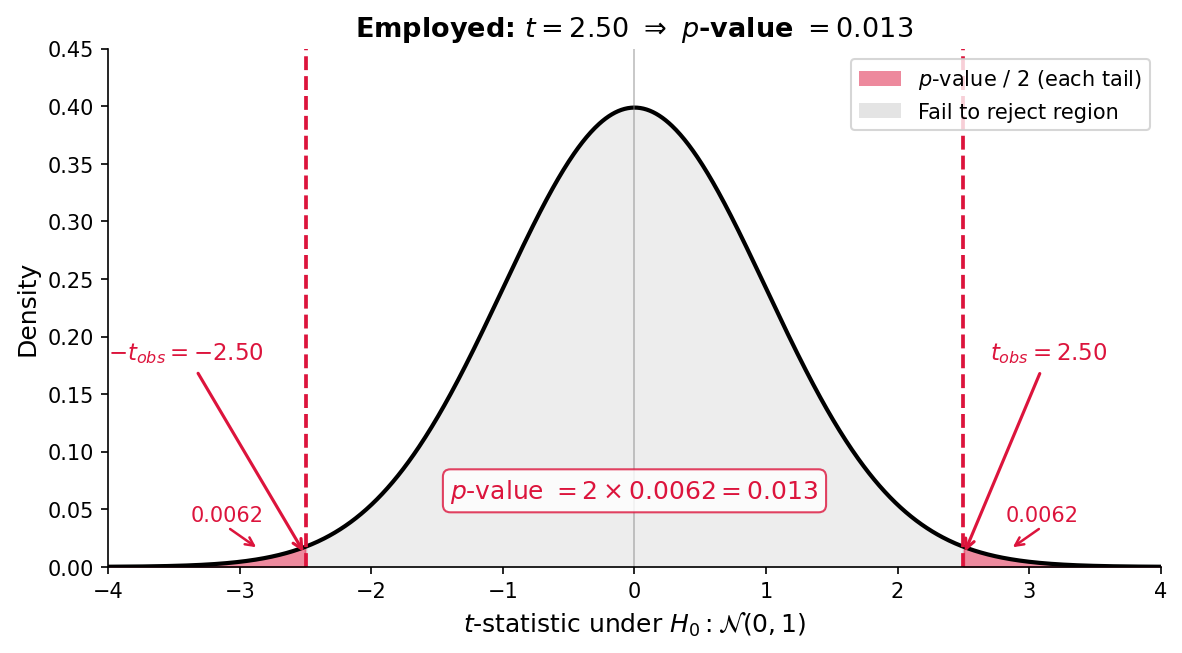
\includegraphics[width=0.90\textwidth]{pvalue_employed.png}
	\end{center}
	\vspace{0.1cm}
	%\begin{itemize}
		%\item Shaded area (both tails) $=$ $p$-value $= 2 \times 0.0062 = 0.013 < 0.05$ $\Rightarrow$ \textbf{reject} $H_0$
	%\end{itemize}
\end{frame}



\begin{frame}{Step 1: Balance Test}{From $t$-statistic to $p$-value}
	%\begin{itemize} 
		
		
		
	%	\item[3.] Evaluate whether the sample estimator is against null hypothesis or not
		\begin{itemize} 
			
	
		\item We usually select an arbitrarily pre-defined threshold value $\gamma$, which is referred to as the \textbf{level of significance}
						\vspace{0.2cm}
		\begin{itemize}	
			%\item The value of $\alpha$ is instead set by the researcher before examining the data
			%\vspace{0.3cm}
			\item By convention, $\gamma$ is commonly set to 0.05 or 0.01
						\vspace{0.2cm}
		\end{itemize}
		%\item If p-value is smaller than $\alpha$, we would say the sample estimate is \textbf{significantly different from the null hypothesis}
		\item \textbf{Decision rule:}
					\vspace{0.2cm}
		\begin{itemize}
			\item If p-value $< \gamma$: \textbf{Reject} the null hypothesis
			\vspace{0.2cm}
			
			\item If p-value $\geq \gamma$: \textbf{Fail to reject} the null hypothesis
		\end{itemize}	
						
		\end{itemize}	
		
		
		
		
		
		
	%\end{itemize}
\end{frame}



\begin{frame}{Step 1: Balance Test}{Reading the Results}
	\begin{itemize}
		\item \textbf{Employed} :
		\vspace{0.2cm}
		\begin{itemize}
			\item $t = 2.50$, $p$-value $= 0.013 < 0.05$ $\Rightarrow$ \textbf{reject} $H_0$
			\vspace{0.2cm}
			\item The two groups are \textbf{significantly different} in employment status
		\end{itemize}
		\vspace{0.2cm}
		\item \textbf{Occ: Consultant} :
		\vspace{0.2cm}
		\begin{itemize}
			\item $t = -0.45$, $p$-value $= 0.655 \geq 0.05$ $\Rightarrow$ \textbf{fail to reject} $H_0$
			\vspace{0.2cm}
			\item \textbf{No significant difference} between the two groups in consultant share
		\end{itemize}
		\vspace{0.2cm}
		\item  In a balance test, we \emph{want} most variables to have large $p$-values 
        		\vspace{0.2cm}

        		\begin{itemize}

        
        \item It means the two groups look similar before treatment
        	\end{itemize}

	\end{itemize}
\end{frame}



\begin{frame}{Step 2: Main Results}{ODO as Causal Effect}
	\begin{center}
		\begin{threeparttable}
			\linespread{1}
			\fontsize{8.5}{8.5pt}\selectfont
			\centering
			\begin{tabular}{@{}lcccc@{}}
				\toprule
				Outcome (Task 2) & Treatment & Control & Diff.\ (ODO) & $p$-value \\
				\midrule\midrule
				Time Spent (min) & 17.0 & 27.0 & \textcolor{red}{$-10.0$} & \textcolor{red}{$<0.001$***} \\
				 & (17.3) & (17.3) & (1.5) & \\
				Average Grade (1--7) & 4.53 & 3.80 & \textcolor{red}{$+0.73$} & \textcolor{red}{$<0.001$***} \\
				 & (1.37) & (1.37) & (0.13) & \\
				\midrule\midrule
				Observations & 218 & 235 & & \\
				\bottomrule
			\end{tabular}
		\end{threeparttable}
	\end{center}
\end{frame}

\begin{frame}{Step 2: Main Results}{Summary}
	\begin{itemize}
		\item ChatGPT significantly reduced task time by 10 minutes ($-37\%$)
		\vspace{0.2cm}
		\begin{itemize}
			\item $p < 0.001$: \textbf{reject} $H_0$ --- the two groups are significantly different
		\end{itemize}
		\vspace{0.2cm}
		\item ChatGPT significantly raised output quality by 0.73 points ($+19\%$)
		\vspace{0.2cm}
		\begin{itemize}
			\item $p < 0.001$: \textbf{reject} $H_0$ --- the two groups are significantly different
		\end{itemize}
		\vspace{0.2cm}
		% \item Both effects are highly significant: a difference this large would occur less than 0.1\% of the time by random assignment alone
		% \vspace{0.3cm}
		\item Because the RCT eliminates selection bias, ODO $=$ ATE
		\vspace{0.2cm}
		\begin{itemize}
			\item ChatGPT \emph{causes} workers to finish faster \emph{and} produce higher-quality output
		\end{itemize}
	\end{itemize}
\end{frame}

\begin{frame}{Additional Results}
	\begin{itemize}
		\item \textbf{Heterogeneous effects:} ChatGPT helped lower-ability workers the most
		\vspace{0.2cm}
		\begin{itemize}
			\item Workers who performed poorly on Task 1 saw the largest improvements on Task 2
			\vspace{0.2cm}
			\item Workers who already performed well maintained their quality while also saving time
			\vspace{0.2cm}
			\item ChatGPT \textbf{compressed the gap} between high- and low-ability workers
		\end{itemize}
		% \vspace{0.3cm}
		% \item \textbf{What makes this credible?}
		% \vspace{0.2cm}
		% \begin{itemize}
		% 	\item Random assignment ensures treatment and control groups are comparable \emph{before} treatment
		% 	\vspace{0.1cm}
		% 	\item Selection bias $= 0$ $\Rightarrow$ the simple difference in means recovers the true causal effect
		% 	\vspace{0.1cm}
		% 	\item Without the RCT, we could not rule out that more productive workers simply chose to use ChatGPT
		% \end{itemize}
		% \vspace{0.3cm}
		% \item \textbf{Bottom line:} ChatGPT raises productivity \emph{and} compresses inequality --- the RCT lets us say this with confidence
	\end{itemize}
\end{frame}



\begin{frame}{Takeaways}
	\begin{itemize}
		% \item \textbf{Heterogeneous effects:} ChatGPT helped lower-ability workers the most
		% \vspace{0.2cm}
		% \begin{itemize}
		% 	\item Workers who performed poorly on Task 1 saw the largest improvements on Task 2
		% 	\vspace{0.1cm}
		% 	\item Workers who already performed well maintained their quality while also saving time
		% 	\vspace{0.1cm}
		% 	\item ChatGPT \textbf{compressed the gap} between high- and low-ability workers
		% \end{itemize}
		% \vspace{0.3cm}
		\item \textbf{What makes this credible?}
		\vspace{0.2cm}
		\begin{itemize}
			\item Random assignment ensures treatment and control groups are comparable \emph{before} treatment
			\vspace{0.2cm}
			\item Selection bias $= 0$ $\Rightarrow$ the simple difference in means recovers the true causal effect
			\vspace{0.2cm}
			\item Without the RCT, we could not rule out that more productive workers simply chose to use ChatGPT
		\end{itemize}
		% \vspace{0.2cm}
		% \item \textbf{Bottom line:} ChatGPT raises productivity \emph{and} compresses inequality --- the RCT lets us say this with confidence
	\end{itemize}
\end{frame}
	
	% \begin{frame}{Step 2: Main Results (Discussion)}
	% 	\begin{itemize}
	% 		\item Because randomization (largely) eliminates selection bias, the \textbf{ODO identifies the ATE}:
	% 		\begin{equation*}
	% 			\underbrace{\mathrm{E}[Y_i | D_i=1] - \mathrm{E}[Y_i | D_i=0]}_{\text{ODO}} \approx \underbrace{\mathrm{E}[Y^1_i - Y^0_i]}_{\text{ATE}}
	% 		\end{equation*}
	% 		\vspace{0.2cm}
	% 		\item \textbf{Time spent:} ChatGPT \emph{reduced} task time by 10 minutes ($-37\%$, from 27 to 17 min)
	% 		\vspace{0.2cm}
	% 		\item \textbf{Output quality:} ChatGPT \emph{raised} average grade by 0.73 points on a 1--7 scale ($+19\%$)
	% 		\vspace{0.2cm}
	% 		\item Both effects are very large: $|t| \approx 7$--$8$, far exceeding any conventional threshold
	% 		\vspace{0.2cm}
	% 		\item \textbf{Conclusion:} ChatGPT simultaneously saves time \emph{and} improves quality --- no tradeoff here
	% 	\end{itemize}
	% \end{frame}
	
	% \begin{frame}{Step 3: The $t$-statistic and $p$-value}
	% 	\begin{itemize}
	% 		\item We observed a 10-minute reduction in time and a 0.73-point improvement in grades --- but could this be \textbf{random chance}?
	% 		\vspace{0.3cm}
	% 		\item \textbf{The null hypothesis ($H_0$):} ChatGPT has no effect; any gap is purely due to luck in random assignment
	% 		\vspace{0.3cm}
	% 		\item The \textbf{$t$-statistic} standardizes the estimated effect relative to its sampling uncertainty:
	% 		\begin{equation*}
	% 			t_{\text{time}} = \frac{-10}{1.3} \approx -7.7, \qquad t_{\text{grade}} = \frac{+0.73}{0.10} \approx +7.3
	% 		\end{equation*}
	% 		\vspace{0.2cm}
	% 		\begin{itemize}
	% 			\item $|t| \approx 7$--$8$ is \textbf{extremely large} --- such gaps would be vanishingly rare under $H_0$
	% 			\vspace{0.2cm}
	% 			\item Compare: under the null, we would expect $|t| < 2$ roughly 95\% of the time
	% 		\end{itemize}
	% 	\end{itemize}
	% \end{frame}
	
	% \begin{frame}{Step 3: The $t$-statistic and $p$-value}
	% 	\begin{itemize}
	% 		\item \textbf{$p$-value:} The probability of observing $|t|$ this large \emph{if $H_0$ were true}
	% 		\vspace{0.3cm}
	% 		\begin{itemize}
	% 			\item $p < 0.001$: less than a \textbf{0.1\% chance} of seeing effects this large by luck alone
	% 			\vspace{0.2cm}
	% 			\item $\Rightarrow$ We \textbf{strongly reject $H_0$}: ChatGPT \emph{causes} faster and better writing
	% 		\end{itemize}
	% 		\vspace{0.4cm}
	% 		\item \textbf{Conventional significance thresholds:}
	% 		\vspace{0.2cm}
	% 		\begin{itemize}
	% 			\item $p < 0.10$: significant at 10\% level \quad ($|t| \gtrsim 1.65$)
	% 			\vspace{0.1cm}
	% 			\item $p < 0.05$: significant at 5\% level \quad ($|t| \gtrsim 1.96$)
	% 			\vspace{0.1cm}
	% 			\item $p < 0.01$: significant at 1\% level \quad ($|t| \gtrsim 2.58$)
	% 		\end{itemize}
	% 		\vspace{0.3cm}
	% 		\item Here, $|t| \approx 7$--$8$ far exceeds any conventional threshold --- both effects are \textbf{highly significant}
	% 	\end{itemize}
	% \end{frame}
	
	% \begin{frame}{Additional Result: Does AI Reduce Inequality?}
	% 	\begin{center}
	% 		\begin{threeparttable}
	% 			\linespread{1}
	% 			\fontsize{8.5}{8.5pt}\selectfont
	% 			\centering
	% 			\begin{tabular}{@{}lcc@{}}
	% 				\toprule
	% 				& Control Group & Treatment Group \\
	% 				\midrule\midrule
	% 				Slope of Task 2 Grade on Task 1 Grade & 0.414 & 0.142 \\
	% 				& & \\
	% 				\midrule
	% 				Difference in Slopes (Treat. $-$ Control) & \multicolumn{2}{c}{$-0.272$} \\
	% 				95\% CI on difference & \multicolumn{2}{c}{$[-0.405, \ -0.140]$} \\
	% 				\midrule\midrule
	% 				Interpretation & \multicolumn{2}{l}{Low-ability workers benefited most from ChatGPT} \\
	% 				\bottomrule
	% 			\end{tabular}
	% 			\begin{tablenotes}
	% 				\fontsize{7}{7pt}\selectfont
	% 				\item Source: Noy \& Zhang (2023), Figure 2. Estimated from regression with grader fixed effects,
	% 				\item clustering SEs at participant level. Slope $=$ coefficient on Task 1 grade.
	% 			\end{tablenotes}
	% 		\end{threeparttable}
	% 	\end{center}
	% \end{frame}
	
	% \begin{frame}{Additional Result: Inequality (Discussion)}
	% 	\begin{itemize}
	% 		\item Did ChatGPT help all workers equally, or disproportionately benefit \textbf{lower-ability} workers?
	% 		\vspace{0.3cm}
	% 		\item The slope of Task 2 grade on Task 1 grade measures \textbf{persistence of initial ability gaps}:
	% 		\vspace{0.2cm}
	% 		\begin{itemize}
	% 			\item \textbf{Control group:} slope $= 0.414$ --- high initial ability predicts high final output
	% 			\vspace{0.2cm}
	% 			\item \textbf{Treatment group:} slope $= 0.142$ --- the initial ability gap is \emph{compressed} by ChatGPT
	% 		\end{itemize}
	% 		\vspace{0.3cm}
	% 		\item The difference in slopes ($-0.272$) is statistically significant (95\% CI excludes zero)
	% 		\vspace{0.3cm}
	% 		\item \textbf{Conclusion:} ChatGPT \emph{reduced} output inequality --- workers who scored low on Task 1 experienced the largest gains in Task 2
	% 		\vspace{0.3cm}
	% 		\item This is consistent with the pattern found across many AI studies: \textbf{novice and lower-ability workers benefit most}
	% 	\end{itemize}
	% \end{frame}
	
	% \begin{frame}{Step 3: Key Takeaway}
	% 	\begin{itemize}
	% 		\item This RCT tells us three things:
	% 		\vspace{0.3cm}
	% 		\begin{itemize}
	% 			\item[1] ChatGPT \textbf{substantially raised productivity}: $-40\%$ time, $+18\%$ output quality
	% 			\vspace{0.3cm}
	% 			\item[2] Effects are \textbf{highly significant} ($p < 0.001$): not noise, but genuine causal effects
	% 			\vspace{0.3cm}
	% 			\item[3] ChatGPT \textbf{reduced inequality}: lower-ability workers benefited more, compressing the grade distribution
	% 		\end{itemize}
	% 		\vspace{0.4cm}
	% 		\item \textbf{The broader lesson:} RCT + hypothesis testing gives us both the \emph{direction} of the causal effect and a measure of our \emph{confidence} in the result
	% 		\vspace{0.3cm}
	% 		\item Without the RCT, we could not separate causation from selection --- maybe workers who \emph{chose} to use ChatGPT are already more productive?
	% 	\end{itemize}
	% \end{frame}
	

	
	\begin{frame}{RCT: The Gold Standard of Causal Inference}
		\begin{itemize}
			\item RCT is widely regarded as the \textbf{gold standard} for causal inference because:
			\vspace{0.2cm}
			\begin{itemize}
				\item It \textbf{directly eliminates} selection bias by design, without relying on modeling assumptions
				\vspace{0.2cm}
				\item Identification rests on \textbf{one transparent assumption}: random assignment
				\vspace{0.2cm}
				\item The simple difference in means is an \textbf{unbiased estimator} of ATE, ATT, and ATU
				\vspace{0.2cm}
				\item Results are \textbf{easy to interpret} and communicate to policymakers
			\end{itemize}
			\vspace{0.3cm}
			\item Other methods (DID, IV, RDD, matching) are often judged by how closely they approximate the ideal of an RCT
		\end{itemize}
	\end{frame}
	
\begin{frame}{Limitations of RCT: Practical Challenges}
	\begin{itemize}
		\item Despite its appeal, RCTs are often \textbf{difficult to implement} in practice:
		\vspace{0.2cm}
		\begin{itemize}
		\item \textbf{Cost:} Running large-scale field experiments requires substantial time and resources
			\vspace{0.2cm}
			\item \textbf{Compliance:} Individuals may not comply with their assigned treatment (non-compliance problem)
			\vspace{0.2cm}
			\item \textbf{Attrition:} Participants may drop out differentially, reintroducing selection bias
			\vspace{0.2cm}
			\item \textbf{Generalizability:} Results from a specific RCT may not generalize to other settings (external validity)
			\vspace{0.2cm}
\item \textbf{Ethics:} Randomly assigning individuals to the control group may be unfair if the treatment is potentially beneficial		\end{itemize}
	\end{itemize}
\end{frame}
	
	% \begin{frame}{Limitations of RCT: Ethical and Practical Impossibility}
	% 	\begin{itemize}
	% 		\item Many important economic and social questions \textbf{cannot be studied using RCTs}:
	% 		\vspace{0.3cm}
	% 		\begin{itemize}
	% 			\item \textbf{Ethical constraints:}
	% 			\vspace{0.1cm}
	% 			\begin{itemize}
	% 				\item Randomly assigning individuals to poverty, unemployment, or smoking is unethical
	% 				\vspace{0.1cm}
	% 				\item Long-run consequences (e.g., childhood deprivation) cannot be experimentally induced
	% 			\end{itemize}
	% 			\vspace{0.3cm}
	% 			\item \textbf{Logistical impossibility:}
	% 			\vspace{0.1cm}
	% 			\begin{itemize}
	% 				\item Macroeconomic policies (monetary policy, trade wars) cannot be randomized across countries
	% 				\vspace{0.1cm}
	% 				\item Historical events, natural disasters, and institutional changes cannot be controlled
	% 			\end{itemize}
	% 			\vspace{0.3cm}
	% 			\item \textbf{Political feasibility:}
	% 			\vspace{0.1cm}
	% 			\begin{itemize}
	% 				\item Governments and firms may resist random policy assignment
	% 			\end{itemize}
	% 		\end{itemize}
	% 	\end{itemize}
	% \end{frame}
	
	% \begin{frame}{When RCT is Not Feasible: Natural Experiments}
	% 	\begin{itemize}
	% 		\item When RCT cannot be conducted, researchers turn to \textbf{quasi-experimental methods} that exploit \textbf{natural experiments}
	% 		\vspace{0.2cm}
	% 		\begin{itemize}
	% 			\item Situations where treatment is ``as good as random'' due to external factors
	% 		\end{itemize}
	% 		\vspace{0.3cm}
	% 		\item Main quasi-experimental strategies:
	% 		\vspace{0.2cm}
	% 		\begin{itemize}
	% 			\item \textbf{Difference-in-Differences (DID):} Exploit policy changes over time
	% 			\vspace{0.2cm}
	% 			\item \textbf{Instrumental Variables (IV):} Exploit exogenous variation that shifts treatment
	% 			\vspace{0.2cm}
	% 			\item \textbf{Regression Discontinuity Design (RDD):} Exploit eligibility cutoffs
	% 			\vspace{0.2cm}
	% 			\item \textbf{Matching:} Control for all observable confounders
	% 		\end{itemize}
	% 		\vspace{0.2cm}
	% 		\item Each method rests on different assumptions --- the key is always to argue why selection bias is eliminated
	% 	\end{itemize}
	% \end{frame}
	
	% \begin{frame}{Summary}
	% 	\begin{itemize}
	% 		\item \textbf{Selection bias} arises because individuals self-select into treatment based on their potential outcomes
	% 		\vspace{0.3cm}
	% 		\item \textbf{RCT} eliminates selection bias by making treatment assignment independent of potential outcomes
	% 		\vspace{0.3cm}
	% 		\item RCT is the \textbf{gold standard} --- but is often impractical or ethically infeasible for many important questions
	% 		\vspace{0.3cm}
	% 		\item Quasi-experimental methods are valuable tools that approximate the ideal of a randomized experiment under carefully stated assumptions
	% 		\vspace{0.3cm}
	% 		\item \textbf{``What's your identification strategy?''} = What assumptions allow you to claim a causal effect?
	% 	\end{itemize}
	% \end{frame}
	
	\begin{frame}{Suggested Readings}
		\begin{itemize}
			\item Chapter 1 and 2, \textit{Mastering Metrics: The Path from Cause to Effect}
			\vspace{0.2cm}
			\item Chapter 2, \textit{Mostly Harmless Econometrics}
			\vspace{0.2cm}
			\item Chapter 4, \textit{Causal Inference: The Mixtape}
		\end{itemize}
	\end{frame}
	
\end{document}